\subsection{Depth variation of isotope ratios --- basic visualization}
\setcounter{step}{0}

\goldbox{}
\begin{minipage}[c]{0.5\textwidth}
During a~NanoSIMS measurement, the sample material is gradually \bb{eroded} by the primary ion beam while the emitted secondary ions are sepa\-rated based on their mass and detected. The ion counts in the subsequent planes therefore record a~\bb{depth} variation of the elements and isotopes within the sample, making it possible to reconstruct their distribution in~3D. This section describes how to use LANS to visualize this 3D variation in the most basic way: by displaying \bb{lateral profiles along depth} in the sample.
\end{minipage}\hfill
\begin{minipage}[c]{0.48\textwidth}
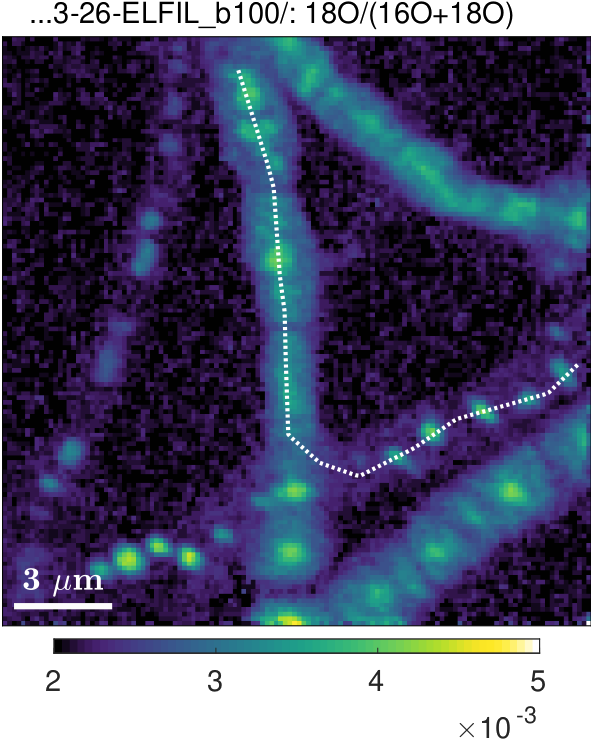
\includegraphics[width=3.5cm, valign=c]{figs3/18O-(16O+18O)-ilp.png}
$\rightarrow$
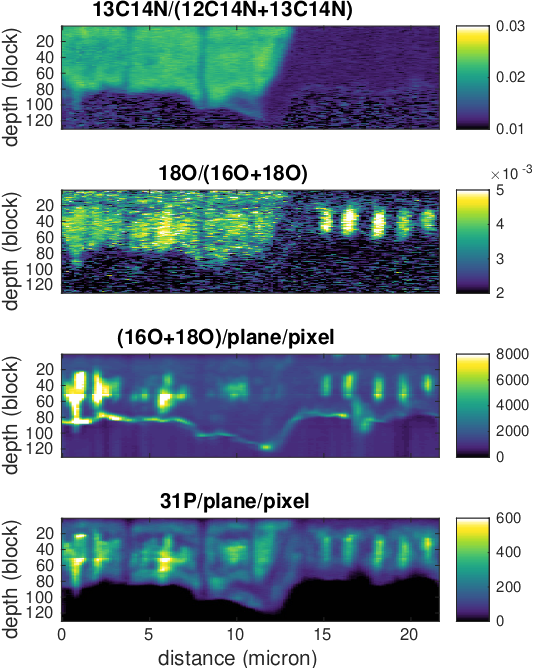
\includegraphics[width=3.5cm, valign=c]{figs3/18O-(16O+18O)-lpd.png}
\end{minipage}

\tcbe

To obtain a~good quality dataset for 3D reconstruction, the measurement needs to use a~relatively low primary ion current to achieve sufficient lateral resolution. At the same time, the same field of view on the sample needs to be measured repeatedly in \bb{many planes} to erode the sample along a~substantial depth interval (several microns) such that a~meaningful 3D variation in this interval occurs. The number of detected planes can start from several hundreds, but it can reach up to several thousands (the example below will use 7000 planes). However, one NanoSIMS measurement in the imaging mode is limited to a~maximum of 1000~planes, which means that the analysis of the same sample area needs to be done as a~\bb{chain} of multiple imaging analyses. This measurement approach leads to multiple raw datasets, which need to be \bb{merged} and analyzed as \bb{one} dataset. Thus, one of the challenges of isotope ratio visualization along depth is the need to load multiple raw datasets and merging them into a~single stack with potentially several thousands of images. 

Another important challenge stems from the fact that because ion count rates for minor isotopes (e.g., ${}^{13}\mathrm{C}$) are typically very low, ion count ratios derived from those minor isotopes (e.g., \ttt{13C/12C}) will generally be noisy if based on data in a~single plane. To maximize the signal-to-noise ratio in depth profiles of isotope ratios while maintaining an acceptable depth resolution, it is better to handle the original ion count data in \bb{blocs} of multiple subsequent planes, where the counts in each bloc are summed up (across the planes but separately for each pixel in the lateral dimension) and treated as \bb{one} plane.  

Overall, basic visualization of the 3D variation in isotope ratios involves three major steps: (i) loading the raw dataset in blocs, possibly involving loading and merging of multiple datasets, (ii) drift-correcting the planes within each bloc before they are summed up into a~single plane, and finally (iii) visualization of lateral profiles along depth. This section describes how to do these processing steps in LANS. 

The example uses data acquired in collaboration with Nicole Geerlings and Filip Meysman, as documented in the following open-access publications:
\skybluebox{}
\begin{center}
\begin{minipage}{0.98\textwidth}
\textsl{\small Geerlings et al.~(2021) Cell Cycle, Filament Growth and Synchronized Cell Division in Multicellular Cable Bacteria. \emph{Front Microbiol}~\bb{12}:620807}. \url{https://doi.org/10.3389/fmicb.2021.620807}
\end{minipage}
\end{center}
\tcbe
\skybluebox{}
\begin{center}
\begin{minipage}{0.98\textwidth}
\textsl{\small Geerlings et al.~(2022) Polyphosphate Dynamics in Cable Bacteria. \emph{Front Microbiol}~\bb{13}:883807}. \url{https://doi.org/10.3389/fmicb.2022.883807}
\end{minipage}
\end{center}
\tcbe

The data is available in the same location as the LANS program (folder \ttt{test\_data/NS+3D}) and includes 7~datasets (\ttt{2020-03-26-ELFIL\_2.im.zip} \dots\ \ttt{2020-03-26-ELFIL\_8.im.zip}) acquired in a~chain of 7~consecutive scans of cable bacteria placed on a~polycarbonate membrane filter. Each dataset comprizes 1000~planes. The first dataset (\ttt{ELFIL\_2}) was acquired using dwell time of 1000\,ms, whereas the remaining datasets used the dwell time of 2000\,ms.

\subsubsection{Loading datasets in blocs, merging multiple datasets}
\setcounter{step}{0}

\s{In preparation for the subsequent steps, first select \lans{Input} $\ra$ \lans{Load raw dataset} to load \bb{all} planes in the first dataset (\ttt{2020-03-26-ELFIL\_2.im.zip}).}

\nnb{This step is required to determine the \lanstf{base mass for alignment} and \lanstf{special region for alignment}, which are necessary later for automatically drift-correcting planes in a~bloc.}

\s{Proceed as described in Sections \ref{sec:display-masses-plane-by-plane} (steps S1--S3) and \ref{sec:drift-correction-accumulation} (steps S1--S2) to define the \lanstf{base mass for} \lanstf{alignment} and \lanstf{special region for alignment}.}

\nb{At this stage, you should \bb{not} proceed with image accumulation (steps S3--S4 in Section~\ref{sec:drift-correction-accumulation}) just yet, because the planes need to be first drift-corrected and accumulated \emph{within} blocs. Instead, proceed as described in the following.}

\sbx{Select \lans{Input} $\ra$ \lans{Load multiple RAW datasets in blocs}. }

\sbx{Navigate to the raw files and select them, using the \ttt{Ctrl} key to select multiple files.}

\nbx{When choosing the analysis of data in blocs, you do \emph{not} necessarily need to load multiple datasets. Indeed, you can choose one dataset if you only want to perform the analysis in blocs just for that one dataset. If you do want to load multiple datasets, however, such as in this example, it is a~prerequisite that they all have the same pixel resolution (e.g., $256\times 256$ pixels).}

\s{In the dialog window that opens, specify the \lanstf{bloc size}, i.e., the number of planes per bloc. If you are going to load data from multiple datasets, indicate whether or not you want to use the same bloc size for all subsequent datasets.}

\nnb{In this example, you will use the bloc size of 100 for the first dataset (\ttt{2020-03-26-ELFIL\_2.im.zip}) and 50 for the other six datasets. This is because the dwell time used to acquire the first dataset was $2\times$ shorter (1\,ms) than the dwell time used for the other datasets (2\,ms). Thus, in the dialog window, first enter 100 in the first field (bloc size) and 0 (\ttt{=no}) in the second field. Then, when loading the subsequent datasets, enter 50 in the first field (bloc size) and 1 (\ttt{=yes}) in the second field.}

\sbx{Click \lans{OK} in the dialog window and observe the progress of loading in the Matlab console.}

\nbx{First, the raw data will be loaded. Then, the drift-correction information for planes in each bloc will be calculated based on the values for \lanstf{Base mass for alignment} and \lanstf{Special region} \lanstf{for alignment} (see Step~2 above). Subsequently, this information will be applied to drift-correct and accumulate planes in blocs for each mass.}

\nnb{If you selected multiple raw datasets, the same steps will be repeated for each of them.}

\nbx{After this step is completed, the dataset loaded in LANS will ``behave'' as any other raw dataset loaded via \lans{Input} $\ra$ \lans{Load RAW dataset}. The only difference will be that each individual plane is, in fact, a~sum of multiple planes (i.e., an accumulated bloc of planes). Thus, the subsequent analysis will proceed according to the same steps as for any other dataset. }

\s{In particular, you need to start with the drift-correction and accumulation of planes via \lans{Input} $\ra$ \lans{Accumulate plane images} (Section~\ref{sec:drift-correction-accumulation}, steps S3--S4).}

\nnb{This is because although the individual planes were drift-corrected \emph{within} each bloc (during the loading process), the drift-correction also needs to be calculated and applied \emph{between} blocs.}

\s{Select \lans{Output} $\ra$ \lans{Save FULL PROCESSED data} to save the image stack, for all masses and all planes, in a~Matlab format (extension \ttt{mat}).}

\nbx{This is highly recommended because the loading of data in blocs, accompanied with drift-correction and accumulation, is quite laborious and may be time consuming. Thus, you likely do not want to do it again for the very same dataset or group of datasets. }

\nnb{When saving the data, use the default filename suggested by LANS, unless you really want to use a~different one. Note that the default filename will end with \ttt{bN.mat}, where \ttt{b} refers to the fact that the data was loaded in blocs and \ttt{N} corresponds to the number of planes per bloc (bloc size). In this example, choose the default filename \ttt{2020-03-26-ELFIL\_b100.mat}.}

\nnb{Beware that if the final dataset contains many planes, the exported \ttt{mat} file may be quite large (e.g., hundreds of MB). Still, this is an acceptable price to pay for not having to load the same multiple datasets in blocs again.}

%%

\subsubsection{Visualization of lateral profiles along depth in the sample}
\setcounter{step}{0}

\goldbox{}
Although you can perform this analysis with any NanoSIMS dataset, it is most useful for datasets that have been loaded in blocs, as described in the previous section.
\tcbe

\sbx{In the main LANS window, select the \lanscb{Display lateral profiles} checkbox in the \ttt{Output options} box.}

\nnb{If you only want to focus on the analysis of lateral profiles, it is a~good idea if you deselect other checkboxes in the \ttt{Output options} box (except for the \lanscb{Export ASCII data} and \lanscb{Export PDF graphics} checkboxes, which should remain selected).}

\sbx{In the \lanstf{expression} and \lanstf{scale} fields, specify the formulas for the ion count ratios you want to analyze and the corresponding scale. }

\nnb{In this example, you will look at depth profiles of ${}^{13}C/({}^{12}C+{}^{13}C)$, ${}^{18}O/({}^{16}O+{}^{18}O)$, $O/plane/pixel$ and $P/plane/pixel$. Thus, enter \ttt{13C14N/(12C14N+13C14N)}, \ttt{18O/(16O+18O)}, \ttt{16O/plane/pixel} and \ttt{31P/plane/pixel} in the expression fields. Then experiment with the optimal scales.}

\nnb{Do not forget to check the corresponding checkboxes next to the formulas.}

\sbx{Select \lans{Output} $\ra$ \lans{Display ratios}. }

\sbx{In the top-left corner of the new window that opens (Fig.~\ref{fig:lateral}A), select the variable based on which you want to define (draw) a~lateral profile.}

\begin{figure}[!ht]
\centering
\begin{tabular}{cc}
A: 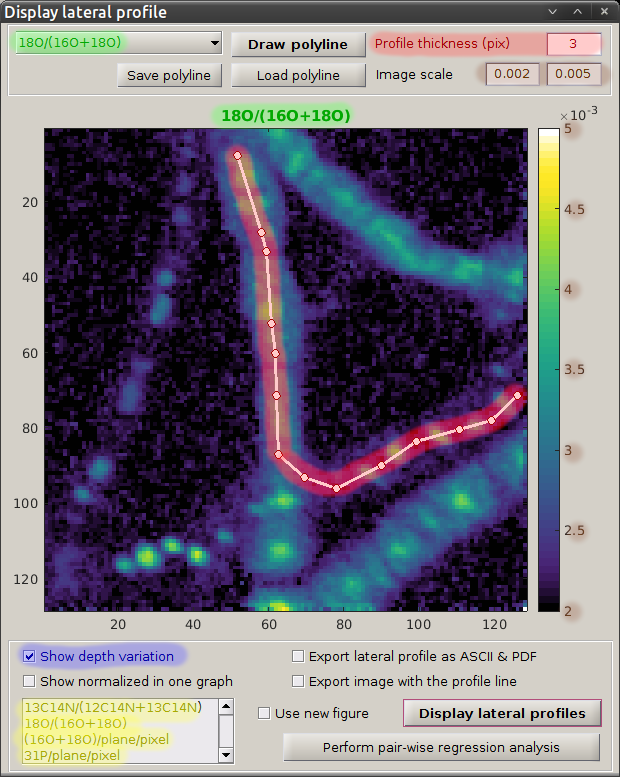
\includegraphics[scale=0.3, valign=t]{figs3/LANS-lateral1}
&
B: 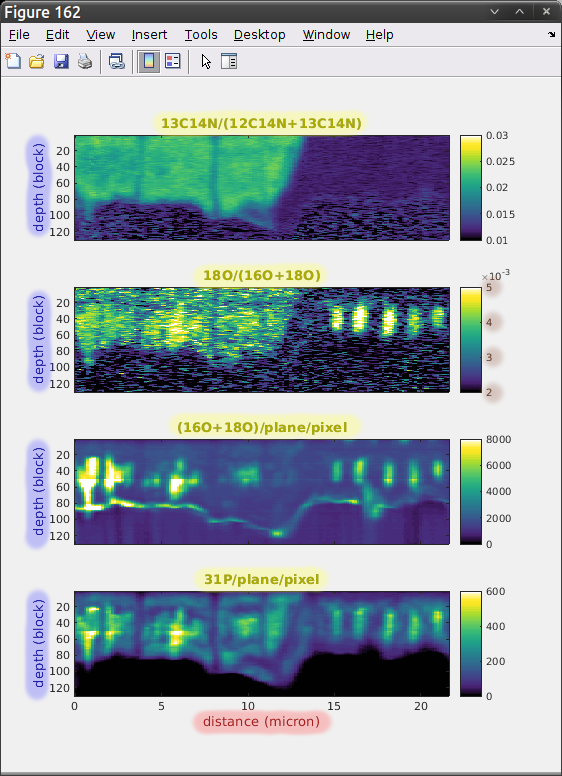
\includegraphics[scale=0.3, valign=t]{figs3/LANS-lateral2}
\end{tabular}
\caption{\label{fig:lateral}%
(A) LANS window for the analysis of variation in ion counts and ion count ratios along a~\bb{lateral} profile. If the \lanscb{Show depth variation} checkbox is selected (marked in blue), the variation along \bb{depth} will also be displayed. Such variations are displayed for all variables selected in the listbox below the checkbox (marked in yellow). The thickness of the lateral profile (red mark) and the color-scale of each variable (brown marks) can also be adjusted. (B) Results of this particular analysis show, among other things, that (i) in the ${}^{13}\mathrm{C}$ non-enriched cells, polyphosphate inclusions, identified as round (oval) areas with markedly higher signals of $P$ and $O$, are significantly and roughly homogeneously enriched in ${}^{18}\mathrm{O}$ relative to the rest of the cell biomass, whereas (ii) the cells enriched in ${}^{13}\mathrm{C}$ show ${}^{18}\mathrm{O}$ enrichment in the polyphospate inclusions as well as in the cytoplasm and DNA.}
\end{figure}

\nnb{In this example, you will look at depth variation in the ${}^{18}O/({}^{16}O+{}^{18}O)$ ratio in polyphosphate inclusions. Thus, select \ttt{18O/(16O+18O)}.}

\sbx{Click on \lans{Draw polyline} to draw a~lateral profile in the image.}

\nbx{The profile can have multiple vertices (hence the name polyline), allowing you to create profiles along a~``curved'' profile or even make sharp corners (Fig.~\ref{fig:lateral}A).}

\nnb{Double-click to define the last vertex of the polyline. Although this will stop the polyline drawing mode, you can still continue adding, moving or removing vertices after this point by clicking with the right mouse button on the polyline. You can also move the entire polyline or remove it and start over.}

\sbx{Specify the \lanstf{Profile thickness}, in pixels.}

\nbx{For the default value of 1, the lateral profile will be based on values in \bb{one} pixel nearest to the polyline. Because this may yield a~rather noisy output, it is recommended to use a~greater value here. For example, using the profile thickness of~5, the lateral profile will be based on values in 5~pixels nearest to the polyline (2~on one side, 2~on the other side, 1~on the polyline). Thus, you can think of the profile as being based on data in a~\bb{band} along the polyline.}

\sbx{Select the \lanscb{Show depth variation} checkbox (highlighted in blue in Fig.~\ref{fig:lateral}A).}

\sbx{In the list of variables (highlighted in yellow in Fig.~\ref{fig:lateral}A), select variables that you want to analyze simultaneously.}

\nnb{Hold \ttt{Ctrl} to select multiple variables. In this example, select all variables.}

\sbx{Click on \lans{Display lateral profiles}.}

\nnb{This will open a new window showing the variation of the selected variables along the lateral profile (`band') and depth (Fig.~\ref{fig:lateral}B), which is the objective of this type of analysis.}

\s{Select the \lanscb{Export} checkboxes and click again on \lans{Display lateral profiles} to export the results as ASCII text and PDF images.}

\sbx{Click on \lans{Save polyline} to save the polyline coordinates.}

\nb{You can load it in the future by clicking on \lans{Load polyline}.}
